\section{Modeling Security Properties with Automata}\label{SecMVA}

This section formally defines the format of the automata that we use
to encode security properties. Our automata are particularly suited to
describe the monitoring of an application, because transitions can
depend on the state of the program being monitored. We call these
automata \emph{Multi-Variable Automata} (MVA), because the internal
state of the automata is defined by a set of variables. Transitions
between states are labelled with guards, events and actions. The event
describes the method that is being called or exited in the monitored
program. Distinction is made between normal and exceptional
terminiation of methods. The guard describes the conditions under
which the transition can be applied. It depends on
\begin{inparaenum}[(\itshape i\upshape)]
\item the automaton state,
\item the program state of the program that is being monitored, and
\item in case the event is method entry, the argument of the method;
in case the event is normal method exit, the result of the method; and
in case the event is exceptional method exit, the exception with which
the method returns.
\end{inparaenum}
The action updates the automaton variables.

Let \(\CP\) and \(\Name\) be an infinite, nonempty sets of control
points and names, respectively.  Throughout, we assume that values can
be booleans, integers, a special null constant, references and or the 
special element of the one element set. \marginnote{How to phrase this?}
Formally:
\[\Val  =  \B(b : \mathbb{B}) \mid \I(i : \mathbb{Z}) \mid \Null \mid
\R(i : \mathbb{Z}) \mid \One \mid \bot
\]
Further, we assume that we have a set of exceptions \Excp, containing
\Throwable, \NullPointer and \JMLExc.


An MVA consists of
\begin{inparaenum}[(\itshape i\upshape)]
\item a name,
\item a class name, to specify which class is being monitored,
\item a finite set of control points,
\item an initial control point,
\item a set of events, to specify which events are being monitored,
\item a set of special MVA variable declarations, to describe
the internal state of the automaton
\item a set of program variable declarations, to specify which
program variables will be inspected by the monitor, and
\item a set of transitions.
\end{inparaenum}
Transitions go from source to target control points. They are labelled
with events, where an event is a tuple of an event type (entry, exit
or exceptional exit) and a method name, and with guards. Each
transition can update the MVA variables by executing a list of
actions, where each action assigns the result of an expression
(containing both program and MVA variables) to a MVA variable. MVA
variables declarations are the same as program field declarations
(defined below), while program variable declarations in the MVA have
the same format as local variable declarations in a program
(\emph{i.e.}, they are not initialised in the
monitor). Figure~\ref{FigMVAForm} shows the main types of the MVA
definition.  We will use a PVS-like notation to declare abstract data
types and records (enclosed by brackets \(\opr\) and \(\clr\)).

\begin{figure}[t]
\[
\begin{array}{rcl}
%\VarDeclA & = \opr & \name : \Name, \type : \Type, \init : \Val \clr\\
%\VarDeclP & = \opr & \name : \Name, \type : \Type \clr\\
\EVENT & = \opr & \etype : (\entry \mid \exit \mid \excexit), 
                 \mname : \Name \clr\\
\TRANS & = \opr & \scp, \tcp : \CP, \event : \EVENT, \\
& & 
\guard : \MVAstate \times \Pstate \times (\Val \mid \Excp) \rightarrow \mathbb{B}, \\
&& \action : (\opr \target : \Name, \expr : \Expr \clr)^* \clr\\
\MVA & = \opr & \name, \clname : \Name, \cps : \setof{\CP},
            \init : \CP, \evs : \setof{\EVENT},\\
     &   &  \vdsA : \setof{\FieldDecl}, \vdsP : \setof{\LocalVarDecl},\\
     &   &  \trans : \setof{\TRANS} \clr
\end{array}
\]
\caption{Formal Definition of MVA}\label{FigMVAForm}
\end{figure}

We require that an MVA is \emph{deterministic}, \emph{i.e.}, for every
source control point and event there is always at most one guard that
holds. Notice that it is not obvious how to transform a
non-deterministic MVA into a deterministic one, because the actions
made by the overlapping transitions might be different. We believe
that this is realistic restriction, and that most important security
properties can be expressed as deterministic MVAs.

An MVA is \emph{total} if there is always exactly one guard that holds
for a given source control point and event, otherwise it is
\emph{partial}. Every deterministic MVA can be completed by function
\complete into a total
MVA. This function adds a special control state
\halted, together with transitions for every control point and every event
to this \halted control point, where the guard is the negation of the
disjunction of all other guards. In addition, one adds unconditional
transitions from \halted to \halted for every possible
event. 

\marginnote{We could give formal definition of completion}
%Formally:
%\[
%\begin{array}[t]{l}
%\mathsf{complete}(a) = 
%\begin{array}[t]{l}
%a \mathsf{with} (\# 
%\begin{array}[t]{l}
%\cps := a.\cps \cup {\halted},
%\trans := a.\trans \cup complete(a.\trans) 
%\end{array}
%\#)
%\end{array}
%\mathsf{complete}(T) =
%\{ (\# \scp := q, 
%       \tcp := \halted,
%       \guard := \lambda s_A s_P v. 
%\end{array}
%\]

\paragraph{MVA Transitions} The state of a MVA consists of a current control
point, and the store of automaton variables.
\[
\MVAstate = \opr \cp : \CP, \stA : \Store \clr
\]
Notice that the program store is not part of the automaton
state. Given a MVA \(a\), the transition function \(\Delta_a\)
describes how given a program store and an event, \(a\) changes its
internal state (where \textit{apply} is a function that updates the
automaton store according to the list of actions in the obvious way).
\[
\begin{array}{l}
\Delta_a  :  \MVAstate \times \Pstate \times \EVENT \hookrightarrow
\MVAstate\\
\Delta_a(\sigma_A, \sigma_P, e) = \\
\quad
\begin{array}[t]{l}
\mathsf{let\ }t = \epsilon(\{t\in \trans(a)\mid
  \begin{array}[t]{l}
     \scp(t) = \cp(\sigma_A) \wedge \event(t) = e \wedge \\
     \guard(t)(\stA(\sigma_A), \st(\fvs(\sigma_P)))\}) \mathsf{\ in}
  \end{array}\\
\quad \opri \cp := \tcp(t), \stA := \mathit{apply}(\action(t),
\stA(\sigma_A)) \clri
\end{array}

\end{array}
\]
In a total MVA, the transition function \(\Delta_a\) is total. Notice
that a partial automaton gets stuck on a certain input if and only if the
complete MVA will reach the state \halted.

\begin{equation}
\Delta_a(s_A, s_P, e) = \perp \Leftrightarrow
\cp (\Delta_{\complete(a)}(s_A, s_P, e)) = \halted
\end{equation}


\paragraph{Example}
Recall the example security automaton in Figure~\ref{FigExample},
expressing that the method \texttt{sendSMS} can
be called at most \(N\) times in between calls to a \texttt{reset}
method. This automaton is formally described by the following
automaton.

\[
\begin{array}[t]{l}
\opri 
\begin{array}[t]{l}
\name := \textrm{LimitSMS}, \clname := \texttt{Messaging},\\
\cps := \{s\},
\init := s,\\
\evs := \{
\begin{array}[t]{l}
\opri \etype := \entry, \mname := \texttt{sendSMS} \clri,\\
\opri \etype := \exit, \mname := \texttt{reset} \clri\},
\end{array}
\\
\vdsA := \{\opri \name := n, \type := \Int, \init := 0 \clri\},
\vdsP := \emptyset,\\
\trans := \{
\begin{array}[t]{l}
\opri 
 \begin{array}[t]{l}
\scp := s, \tcp := s, 
             \event := \opri \etype := \entry, 
                             \mname := \texttt{sendSMS} \clri, \\
             \guard := \lambda(s_A, s_P, v). n(s_A) < N,
             \action := \opri \target := n, \expr := n + 1 \clri 
            \clri,
\end{array}\\
\opri 
\begin{array}[t]{l}
\scp := s, \tcp := s,
             \event := \opri \etype := \exit, \mname := \texttt{reset}
\clri, \\
             \guard := \ttt, 
             \action := \opri \target := n, \expr := 0 \clri
           \clri \}
\end{array}
\end{array}
\end{array}\\
\clri
\end{array}
\]

Completion would add a transition from \(s\) to the new state \halted
for the event that \texttt{sendSMS} is entered, with a guard \(n \geq
N\). For the exit event of \texttt{reset}, the transition to halted
would have a guard \fff. And of course, there would be an unguarded
transition from \halted to \halted. Figure~\ref{FigCompleteMVA} shows
the complete MVA. 
 
\begin{figure}[t]
\begin{center}
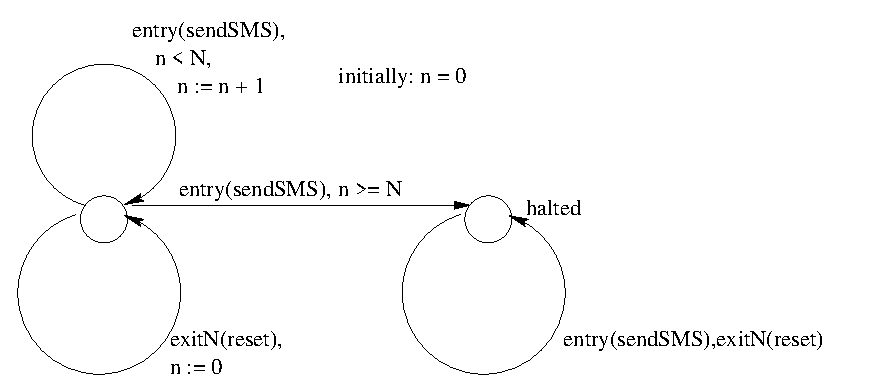
\epsfig{file=completed.eps, width=4cm}
\end{center}
\caption{Automaton of Figure~\ref{FigExample}, after completion}
\end{figure}
